\chapter{基于显著锚点几何嵌入的点云配准}
\thispagestyle{others}
\pagestyle{others}
\xiaosi

    \section{本章引言}
    随着三维捕获传感器的出现,点云的采集变得越来越方便。许多行业都受益于点云的利用,如自动驾驶\upcite{Temporal, L3Net, IMLSSLAM}、机器人\upcite{Positioning}、虚拟现实\upcite{Generative_Adversarial,Single_Image}和形状建模\upcite{LPOT, Birds_Stone}。
    由于三维传感器的视野有限,在应用中经常需要将若干部分点云对齐到同一个坐标系下形成完整的视图。
    传统点云配准主要依靠经典优化策略的对应搜索和迭代变换估计。
    传统的配准方法对未知场景具有较好的泛化能力,但容易受到噪声、异常值、部分重叠和不同密度等因素的影响,而这种缺陷在实际扫描的点云中普遍存在。

    随着深度学习的蓬勃发展,许多方法\upcite{INENet,Task_specific,RANSAC_Hypotheses}通过神经网络学习到的特征进行对应搜索,并通过鲁棒性变换估计完成变换矩阵的预测。有些方法\upcite{Graphite}则根据学习到的特征,对源点云和目标点云中的关键点进行检测和匹配,并完成配准。最近的由粗到细的点云配准方法表现出优越的性能\upcite{CoFiNet}。首先通过聚合原始点获得超点并提取超点特征,然后在特征空间中寻找另一帧中的最近点形成超点对应。超点在空间中表示一个连续的几何区域,根据超点对应可以在相应区域内进一步通过特征最近点寻找到点对应关系,最后根据点对应完成最终的变换估计。Geo\upcite{Geometric}利用注意力机制\upcite{Attention}将全局上下文合并为特征,可以得到更好的超点匹配。给定一个超点,所有其它超点的几何信息被无差别地嵌入到特征中。然而,点云通常存在弱几何区域和重复图案。在这种情况下,周围的区域往往充满了相似的几何结构,而模糊的几何结构的加入,并不能帮助区分弱几何和重复图案区域的超点。

    由于源点云与目标点云之间存在非重叠区域的重复图案以及重叠区域的弱几何区域两种具有几何挑战的情况,因此精确提取源点云与目标点云之间的点对应并非易事。图\ref{fig:example}展示了本章方法与Geo在具有几何挑战性的情况下两个例子的区域对应和点对应关系:第一行是本方法的区域对应和点对应可视化;第二行是Geo的区域对应和点对应的可视化;第一列和第三列是两种方法的区域对应;第二列和第四了是两种方法的点对应。图中绿线表示正确的对应,红线为错误的对应。第一个例子是非重叠区域存在重复图案的情况,源点云和目标点云包含相似的沙发,这些沙发在不重叠的区域外观相似。可以观察到由于重复图案,Geo方法在沙发上提取了大量的错误匹配。此外,对于重叠区域的弱几何区域而言因为可以提取的特征很少,也很难获得准确的对应关系。如第二个例子所示,地板由平面组成,而平面自身的几何结构并不具备差异性这也导致了平面内部超点特征的相似。由于内部特征相似,因此Geo也不能提取正确的的对应关系。这些问题对定位精确的点对应并进行可靠的配准提出了巨大的挑战,在室内情况下尤其突出。
    % (1)非重叠区域的重复模式和(2)重叠区域的低几何区域。

    \begin{figure}[h]
        \centering
        \includegraphics[width = \textwidth]{my/figure/3-1.pdf}
        % \captionsetup{margin = {1.6cm,1.6cm}}
        \bicaption[\xiaosi 第三章方法和Geo在具有几何挑战性的情况下的对比]{\wuhao 本方法和Geo在具有几何挑战性的情况下的对比。}{\wuhao Comparison of our method and Geo in geometrically challenging situations. }
        \label{fig:example}
    \end{figure}
    \vspace{-0.35cm}

    因此,在本章中,提出了一种鲁棒点云配准方法。一组包含相对丰富的判别几何信息的超点对应被定位为显著锚点对应,显著锚点对应由锚点定位模块产生。由于正确的超点对应与这组显著锚点对应存在几何空间一致性,因此将超点与显著锚点之间的几何进行嵌入可以有效地剔除异常值。又由于相似非重叠区域超点以及弱几何区域超点相对于这组锚点的几何位置不同,因而其几何特征也会存在差异,因此将锚点与超点的几何特征进行嵌入能够有效增加上述两种情况超点间的差异性,使得模型能够在几何挑战较大的区域获得准确的点对应。该方法不仅能够提高点云配准的准确性,还能够有效处理异常值和几何挑战较大的情况,具有广泛的应用前景。

    具体来说,本章节首先设计了一个锚点定位模块,利用非极大值抑制法来获取源点云和目标点云上分布稀疏且保持一定几何结构的锚点对应。通过显著锚点,本方法提出了一种选择性几何嵌入模块,增强了超点特征间的差异性,以实现精确的超点匹配。本研究利用注意力机制,有选择地嵌入锚点的几何信息,而不是聚集周围超点的所有几何信息。利用交叉注意力机制,将锚点-超点的距离和角度嵌等选择性几何信息入。为了获取最有效的锚点和显著特征,迭代更新锚点的位置和超点特征,这对于获得精确的超点对应关系起着至关重要的作用。最后,利用姿态估计器通过点的对应关系来生成最终的变换矩阵。\par
    (1)提出了一个健壮的点云配准框架,通过嵌入显著性锚点的几何结构,能够实现具有弱几何结构和重复图案的点云配准的最先进性能。
    (2)设计了一种选择性几何结构嵌入方法,通过在超点和显著锚点之间嵌入几何信息来增强超点特征的区别。
    (3) 提出了一种锚点定位和更新方法,以获得在源点云和目标点云的重叠区域中分布稀疏且包含丰富的判别几何信息的最有效的锚点。

    \section{基于显著锚点几何嵌入的点云配准方法}
    \subsection{问题陈述}
    给定来自不同视角的且部分重叠的源点云$\mathcal{P}=\{{\mathbf{p}_i} \in \mathbb{R}^{3} \mid i=1,..,N\}$和目标点云$\mathcal{Q}=\{{\mathbf{q}_j} \in \mathbb{R}^{3} \mid j =1,\dots,M\}$,点云配准的目标是求解变换矩阵$\mathbf{Trans}$使得两点云对齐。$\mathbf{Trans}$由旋转矩阵$\mathbf{R}$和平移向量$\mathbf{t}$组成,数学描述由公式(3-1)表示:
    \begin{equation}
        \mathrm{arg}\underset{\mathbf{R}, \mathbf{t}}{\min} \sum_{(\mathbf{p}_i, \mathbf{q}_j) \in \mathcal{C}} 
        {\left\|{\mathbf{q}_j-(\mathbf{R} \cdot \mathbf{p}_i+\mathbf{t})}\right\|_{2}^{2}}
    \end{equation}
    式中,$(\mathbf{p}_i, \mathbf{q}_j)$属于集合$\mathcal{C}$,表示源点云的$\mathbf{p}_i$点和目标点云的$\mathbf{q}_j$是一对对应点。如第二章所述,求解变换矩阵的问题转换为了寻找对应关系集合$\mathcal{C}$的问题。

    \subsection{方法概述}
    如图\ref{fig:framework}所示,在使用共享骨干网络提取点云特征后,本方法首先使用所提出的锚点定位模块在源点云和目标点云中定位初始锚点对应关系。在选定锚点的基础上,结合锚点的几何特征,提出了选择性几何嵌入模块,增强了超点特征的区分性。为了获得最显著的锚点和差异性的超点特征,提出了一种基于迭代优化的显著锚点更新(IOSAU)方法,以迭代方式更新锚点位置和超点特征。通过迭代增强特征差异性,可以实现精确的超点匹配。然后在每个超点内获得可靠的点对点的对应关系。最后,利用姿态估计器获得变换矩阵并进行精确配准。

    \vspace{-0.1cm}
    \begin{figure}[h]
        \centering
        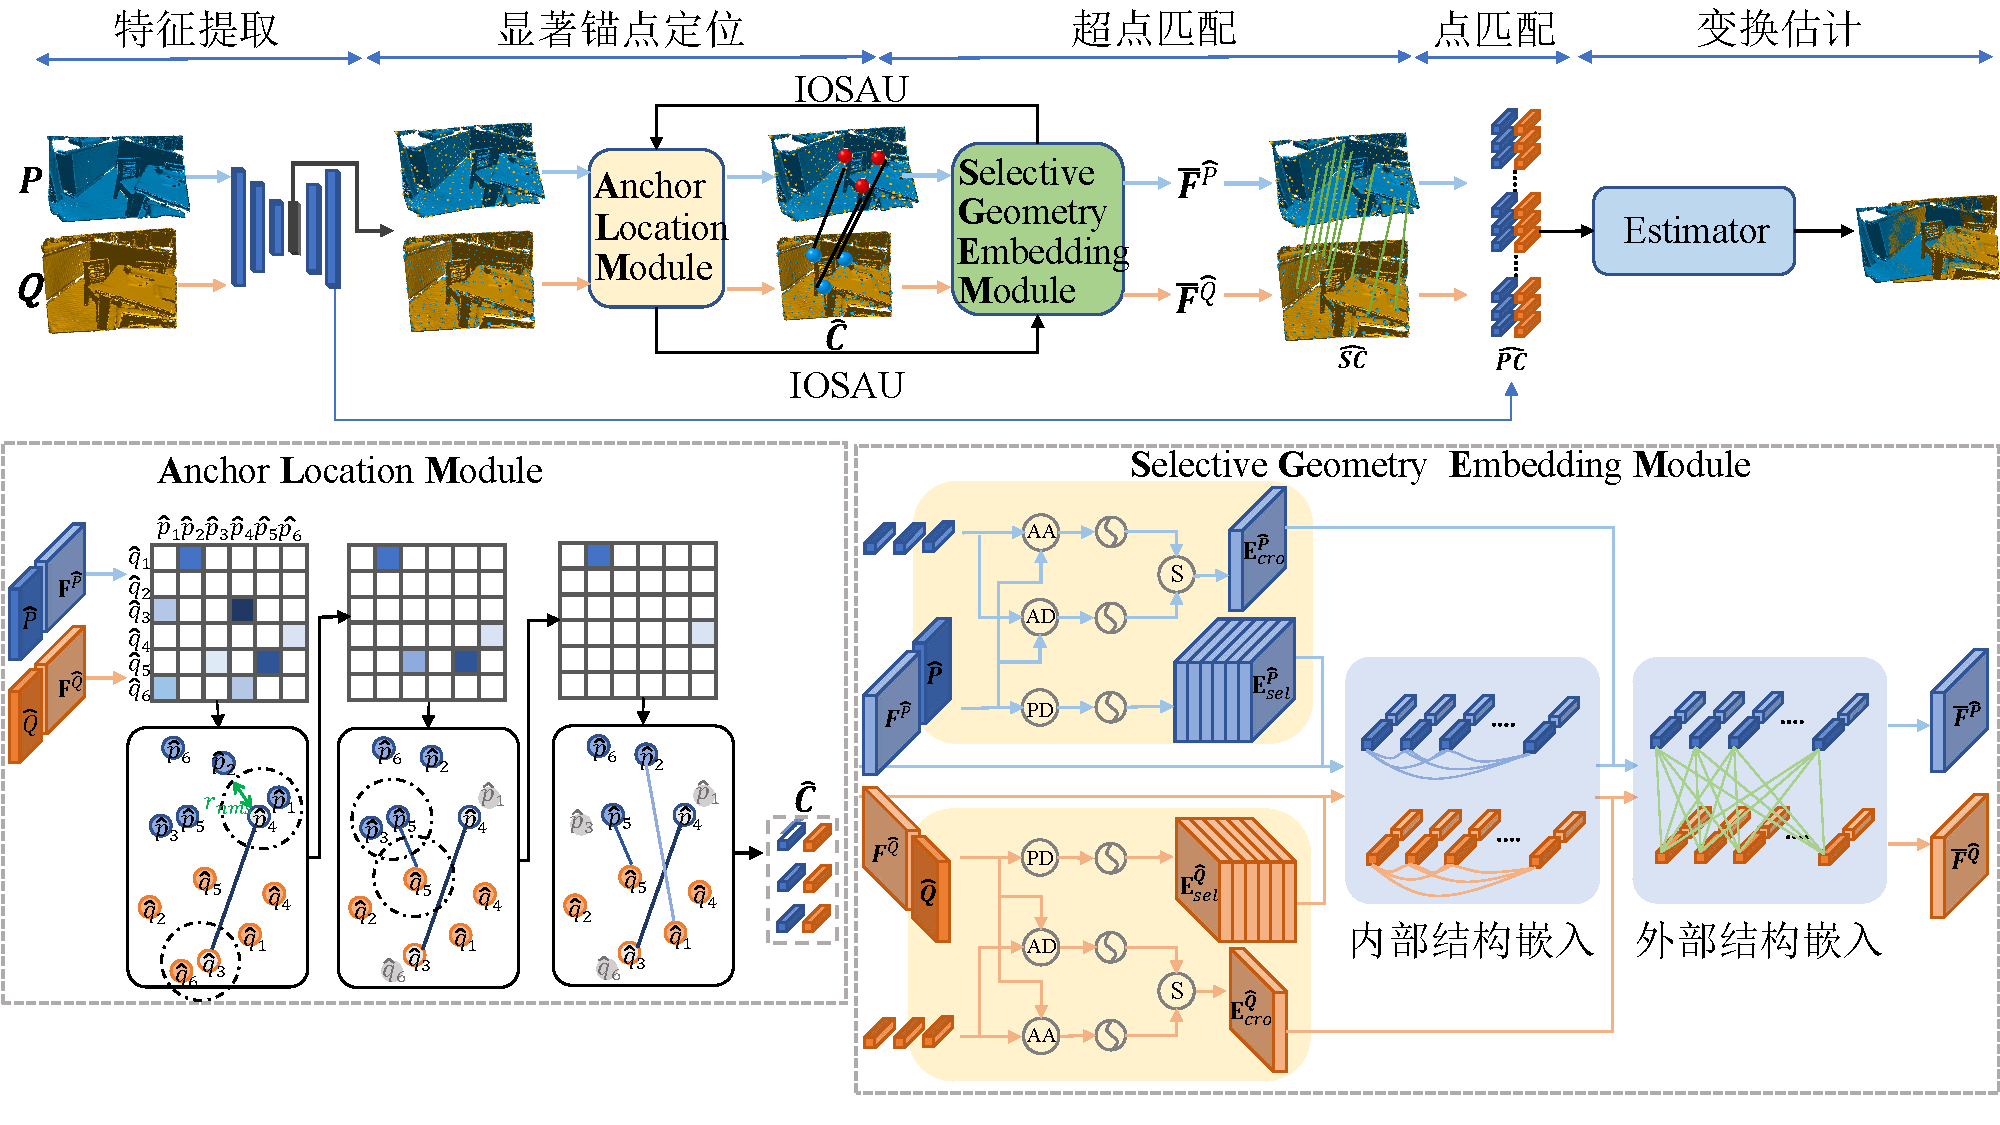
\includegraphics[width = \textwidth]{my/figure/3-2.pdf}
        \bicaption[\xiaosi 第三章点云配准方法概述]{\wuhao 本点云配准方法概述}{\wuhao Overview of the proposed registration method}\label{fig:framework}
    \end{figure}
    \vspace{-0.35cm}

    \subsection{锚点定位模块}
    本研究首先将源点云$\mathcal{P}$和目标点云$\mathcal{Q}$送入共享骨干网络KPConv中。在这个网络中原始点云将被下采样为超点并提取特征,本文用符号$\mathcal{\hat{P}} = \{\mathbf{\hat{p}}_i\}_{i=1}^{|\mathcal{\hat{P}}| }$和$\mathcal{\hat{Q}} = \{\mathbf{\hat{q}}_j\}_{j=1}^{|\mathcal{\hat{Q}}| }$分别表示源点云和目标点云的超点,用符号$\mathbf{F}^{\hat{\mathcal{P}}} \in \mathbb{R}^{\left|\mathcal{\hat{P}}\right| \times \hat{d}}$和$\mathbf{F}^{\hat{\mathcal{Q}}} \in \mathbb{R}^{\left|\mathcal{\hat{Q}}\right| \times \hat{d}}$分别表示这些超点的特征。下采样和特征提取过程可以表述为:
    $\left(\mathbb{R}^{\left|\mathcal{P}\right|\times 3},
    \mathbb{R}^{\left|\mathcal{Q}\right|\times 3}\right) 
    \rightarrow 
    \left(\mathbb{R}^{\left|\hat{\mathcal{P}}\right| \times \hat{d}}, 
    \mathbb{R}^{\left|\hat{\mathcal{Q}}\right| \times \hat{d}}\right)$,其中$ \hat{d}$表示超点特征的通道数。\par

    \vspace{-0.1cm}
    \begin{algorithm}[h]
        \caption{锚点定位}
        \label{alg:anchor_location}
        \LinesNumbered 
        \KwIn{抑制半径$r_{nms}$, 相似矩阵$\mathbf{S}$, 锚点个数$K$}
        \KwOut{$\mathcal{\hat{C}} = \{(\mathbf{\hat{a}}_k,\mathbf{\hat{b}}_k) \mid k=1,\dots,K\}$。其中$\mathbf{\hat{a}}_k$、$\mathbf{\hat{b}}_k$分别表示第$k$个锚点对应在源点云和目标点云中的坐标。}
    
        $\mathcal{\hat{C}} = \phi$ \\
        \While{$|\mathcal{\hat{C}}|<K$}{
            $S_{i,j}=max(\mathbf{S})$; \\
            $\mathcal{\hat{C}} = \mathcal{\hat{C}} \cup (\mathbf{\hat{p}}_{i}, \mathbf{\hat{q}}_{j})$; \\
                \For{$x \in \{1,2,...,row(\mathbf{S})\}$}{
                \If{$||\mathbf{\hat{p}}_{i}-\mathbf{\hat{p}}_{x}||_2<r$}{
                    remove($\mathbf{S}_{x,-}$)
                }
            }
                \For{$y \in \{1,2,..., col(\mathbf{S})\}$}{
                \If{$||\mathbf{\hat{q}}_{j}-\mathbf{\hat{q}}_{y}||_2<r$}{
                    remove($\mathbf{S}_{-,y}$)
                }
            }
        }
    \end{algorithm}
    \vspace{-0.35cm}

    在获取超点后,本方法再定位源点云和目标点云中保持一定几何结构的的锚点对应。一旦得到可靠的锚点对应,就可以将它们作为参考点,将锚点与超点之间的几何结构信息嵌入到每个超点特征中。这样就可以消除特征相似导致的错误超点匹配。因此,在锚点定位模块中,本模块的目标是获取那些具有判别特征的超点对应作为显著锚点对应。\par

    给定源点云和目标点云的超点特征$\mathbf{F}^{\hat{\mathcal{P}}}$和$\mathbf{F}^{\hat{\mathcal{Q}}}$,初始锚点对应可以选择在相似矩阵$\mathbf{S}$中具有较高置信度的超点对应。如图\ref{fig:framework}所示,为了获得分布稀疏的保持一定几何结构的锚点对应,本方法放弃了传统的Top-K选择方法,即连续选择几个最高置信度的超点匹配,避免了所选锚点对应关系位置集中。原因是因为当这组锚点存在聚集情况时,在后续几何嵌入过程中聚集的多个锚点就会退化为一个锚点。对于一个锚点而言,无论是角度还是距离,不同超点与它之间的结构差异性就会丢失。因此,本模块采用非最大值抑制\upcite{NMS}(Non-Maximum Suppression,NMS)来保证所选锚点对应的空间均匀性和稀疏性。首先利用$\mathbf{F}^{\hat{\mathcal{P}}}$和$\mathbf{F}^{\hat{\mathcal{Q}}}$计算源点云和目标点云的超点之间的相似分数矩阵,并从置信度最高到最低进行排序。非最大抑制应用于每个超点周围的固定半径$r_{nms}$。在选择最高置信度的超点后,去除所有在$r_{nms}$的欧氏距离内的对应关系。在剩余的超点中,本模块选择置信度最高的对应作为第二锚点对应,并删除位于$r_{nms}$半径内的对应。重复这个过程,直到本模块获得$K$个初始锚对应,定义如公式(3-2)所示:
    \begin{equation}
        \hat{\mathcal{C}}=\{(\mathbf{\hat{a}}_k,\mathbf{\hat{b}}_k) \mid k =1,\dots,\mathrm{K}\}
    \end{equation}
    式中,$\mathbf{\hat{a}}_k$、$\mathbf{\hat{b}}_k$分别表示第$k$个锚点对应在源点云和目标点云中的坐标。算法\ref{alg:anchor_location}描述了锚点定位的整个过程。

    \subsection{选择性几何嵌入模块}
    在提出的选择性几何嵌入模块中,融合了锚点和超点之间的几何信息。每个点云内部的超点距离通过自注意机制嵌入到超点特征中。在两个点云信息交流过程中,本模块将超点与所有锚点之间的角度和距离进行编码,并与超点的特征进行融合。本方法没有直接将一个点云上的所有超点信息聚合到另一个点云上,而是有选择地嵌入相应锚点的几何信息,进一步增强了超点特征的显著性。将锚点的几何形状嵌入有以下几个优点:(1)在源点云和目标点云只有部分重叠的情况下,直接交换两个点云的所有信息会不可避免地会引入噪声和扰动;(2)有选择地嵌入稀疏和正确的锚点几何,可以避免弱几何区域的对称、上下和前后翻转问题。\par
    本模块为每个点云构造锚点与超点间的距离和角度。当锚点匹配时,正确对应的超点具有一致的锚点距离和角度。为此,本模块利用交叉注意机制将这种几何一致性合并到超点特征中,从而实现点云几何信息的交换。通过这种方式,本模块的选择性几何嵌入模块能够帮助匹配更精确的超点对应。\par

    \subsubsection{内部结构嵌入}
    点云内部结构包含上下文全局信息,有利于增加超点特征间的区分度。在自注意机制中,本模块明确地将超点间的距离信息嵌入到点云特征中。下面本文将以以源点云为例详细说明内部结构嵌入的整个过程。
    给定源点云中的一个超点$\mathbf{\hat{p}}_{i}$,本模块首先计算超点$\mathbf{\hat{p}}_{i}$与其他任意超点$\mathbf{\hat{p}}_{i}$之间的距离,并根据超参数$\sigma_{d}$调节二者的距离灵敏度,随后利用正弦函数将$\mathbf{\hat{p}}_{i}$与$\mathbf{\hat{p}}_{i}$的距离这一标量映射到高维空间,具体流程由公式(3-3)表示:
    \begin{equation}
        \centering
            \mathbf{E}_{sa}^{\mathcal{\hat{P}}_{(i,j)}} = f(d(\mathbf{\hat{p}}_{i},\mathbf{\hat{p}}_{j})/\sigma_{d})
    \end{equation}
    式中,$d(\mathbf{\hat{p}}_{i},\mathbf{\hat{p}}_{j})=\left\|{\mathbf{\hat{p}}_{i}-\mathbf{\hat{p}}_{j}}\right\|_{2}^{2}$表示超点$\mathbf{\hat{p}}_{i}$和$\mathbf{\hat{p}}_{j}$之间的距离;$\sigma_{d}$是调节距离灵敏度的系数,一般设置在$0.1\sim 0.5$之间;$f(\cdot)$表示一个正弦函数,它将标量映射到高维特征。

    给定超点特征$\mathbf{F}^{\mathcal{\hat{P}}}$和距离编码$\mathbf{E}_{sa}^{\mathcal{\hat{P}}}$,利用自注意力机制将超点特征与超点距离编码进行融合。
    利用三个可学习矩阵$\mathbf{W}_{q}$,$\mathbf{W}_{k}$和$\mathbf{W}_{v}$分别将$\mathbf{F}^{\mathcal{\hat{P}}}$映射为$\mathbf{F}_{q}^{\mathcal{\hat{P}}}$、$\mathbf{F}_{k}^{\mathcal{\hat{P}}}$和$\mathbf{F}_{v}^{\mathcal{\hat{P}}}$。
    $\mathbf{W}_{g}$用来将$\mathbf{E}_{sa}^{\mathcal{\hat{P}}}$映射到$\mathbf{E}_{g}^{\mathcal{\hat{P}}}$。然后利用$\mathbf{F}_{q}^{\mathcal{\hat{P}}}$、$\mathbf{F}_{k}^{\mathcal{\hat{P}}}$、$\mathbf{E}_{g}^{\mathcal{\hat{P}}}$计算相似度矩阵$\mathbf{Score}$,其中矩阵每一行每一列的值由公式(3-4)计算:
    \begin{equation}
        \centering
        \mathbf{Score}_{(i, j)}= 
        \frac{
        \mathbf{F}_{q}^{\mathcal{\hat{P}}_{i}} \cdot (\mathbf{F}_{k}^{\mathcal{\hat{P}}_{j}} + \mathbf{E}_{g}^{\mathcal{\hat{P}}_{(i, j)}})^\mathrm{T}
        }{\sqrt{\hat{d}}}
    \end{equation}
    融合点云自身结构信息后的超点特征$\mathbf{F}^{\mathcal{\hat{P}}}$可由公式(3-5)计算得到:
    \begin{equation}
        \centering
        \mathbf{F}^{\mathcal{\hat{P}}} =softmax(\mathbf{Score}) \cdot \mathbf{F}_{v}^{\mathcal{\hat{P}}}
    \end{equation}\par

    \subsubsection{外部结构嵌入}
    两点云之间的信息交流在点云配准问题中起着至关重要的作用,特别是在低重叠的情况下。即使通过自我注意力机制嵌入了自身的几何图形,由于源点云和目标点云中普遍存在重复的图案,仍然存在区域特征相似的情况。对于这些超点,相似的特征会导致源点云和目标点云之间的不匹配。因此,需要在目标点云和源点云之间通过显著锚点对应进行信息交换。与Geo方法不加区别地使用交叉注意力融合另一帧点云特征的方式不同,本模块采用一种选择性几何嵌入方法,构建锚点和超点之间的结构编码,然后将源点云和目标点云信息进行交流。其过程如图\ref{fig:cross_attention}所示。源点云和目标点云的超点的特征和几何结构使用交叉注意机制显式地融合。\par

    \vspace{-0.1cm}
    \begin{figure}[htp]
        \centering
        \includegraphics[width = 8.5cm]{my/figure/3-3.pdf}
        \bicaption[\xiaosi 交叉注意力的计算图]{\wuhao 交叉注意的计算图}{\wuhao The computation graph of cross-attention}
        \label{fig:cross_attention}
    \end{figure}
    \vspace{-0.35cm}

    对于源点云中的某个超点$\hat{\mathbf{p}}_{n}$,$\{\hat{\mathbf{a}}_i\}_{i=1}^K$表示为锚点集合,本模块用公式(3-6)计算上超点与第$i$个锚点之间的距离:
    \begin{equation}
        \rho_{i} = d(\hat{\mathbf{p}}_{n},\hat{\mathbf{a}}_i)
    \end{equation}
    然后同内部结构嵌入一致,使用$f(\cdot)$函数将锚点与超点的距离映射到高维特征。然后根据锚点对应得分进行加权求和,形成超点距离编码如公式(3-7)所示:
    \begin{equation}
        \mathbf{Ed}_{ca}^{\mathcal{\hat{P}}_{n}}=  \sum_{i=1}^{K} {f(\rho_{i})/\sigma_{d}}
    \end{equation}
    式中,$\mathbf{Ed}_{ca}^{\mathcal{\hat{P}}_{n}}$是锚点-超点距离嵌入;$K$表示锚点数量;$\sigma_{d}$是用于调节距离灵敏度的参数。除了距离嵌入,超点与锚点之间的角度也被融合到特征中。如图\ref{fig:embedding}所示,本方法以$\hat{\mathbf{p}}_n$为顶点。顶点和两个锚点组成一个夹角,定义为公式(3-8):
    \begin{equation}
        \centering
        \theta_k(\mathbf{\hat{p}}_n, \mathbf{\hat{a}}_l, \mathbf{\hat{a}}_s)= deg(\mathbf{\hat{a}}_l-\mathbf{\hat{p}}_n,\mathbf{\hat{a}}_s - \mathbf{\hat{p}}_n)
    \end{equation}
    式中,$\theta$表示锚点与超点之间角度;$\mathbf{\hat{a}}_l$表示源点云中的第$l$个锚点;$\mathbf{\hat{a}}_s$表示源点云中的第$s$个锚点;$deg(\cdot)$表示计算角度的度函数。在获得锚点与超点的夹角后,本模块使用正弦函数$f(\cdot)$将其映射到高维特征。然后利用置信度加权和得到超点的角度编码,如公式(3-9)所示:
    \begin{equation}
        \mathbf{Ea}_{ca}^{\mathcal{\hat{P}}_{n}} = \sum_{k = 1}^{C_K^2} f(\theta_k(\mathbf{\hat{p}}_{n}, \mathbf{\hat{a}}_l, \mathbf{\hat{a}}_s)/\sigma_\theta)
    \end{equation}
    式中,$K$为锚点的个数;$C_K^2$为组合的个数;$\sigma_\theta$是调节角度灵敏度的系数。然后,将超点距离编码$\mathbf{Ed}_{ca}^{\mathcal{\hat{P}}_n}$与超点角度$\mathbf{Ea}_{ca}^{\mathcal{\hat{P}}_n}$相加,利用公式(3-10)得到最终的超点几何编码:
    \begin{equation}
        \mathbf{E}_{ca}^{\mathcal{\hat{P}}_{n}} =  \mathbf{Ed}_{ca}^{\mathcal{\hat{P}}_{n}} + \mathbf{Ea}_{ca}^{\mathcal{\hat{P}}_{n}}
    \end{equation}

    上述锚点与超点间的几何结构嵌入过程如图\ref{fig:embedding}所示,首先计算出锚点与超点之间的距离和角度,并进行编码,随后将角度和距离编码进行信息合并,形成最终的几何编码。对于目标点云中的超点$\mathbf{\hat{q}}_m$,可以用同样的方法得到几何编码,记为$\mathbf{E}_{ca}^{\mathcal{\hat{Q}}_m}$。\par

    利用KPConv提取的超点特征$\mathbf{F}^{\mathcal{\hat{P}}_n}$和$\mathbf{F}^{\mathcal{\hat{Q}}_m}$,以及在源点云和目标点云中几何编码$\mathbf{E}_{ca}^{\mathcal{\hat{P}}_{n}}$和$\mathbf{E}_{ca}^{\mathcal{\hat{Q}}_{m}}$,通过交叉注意力技术进行融合。
    本方法利用可学习的矩阵$\mathbf{W}_q$将$\mathbf{F}^{\mathcal{\hat{P}}_n}$映射到$\mathbf{F}_{q}^{\mathcal{\hat{P}}_n}$,利用可学习的矩阵$\mathbf{W}_k$和$\mathbf{W}_v$将$\mathbf{F}^{\mathcal{\hat{Q}}_m}$映射到$\mathbf{F}_{k}^{\mathcal{\hat{Q}}_m}$和$\mathbf{F}_{v}^{\mathcal{\hat{Q}}_m}$,利用可学习的矩阵$\mathbf{W}_g$将$\mathbf{E}_{ca}^{\mathcal{\hat{P}}_{n}}$和$\mathbf{E}_{ca}^{\mathcal{\hat{Q}}_{m}}$映射到$\mathbf{E}_{g}^{\mathcal{\hat{P}}_{n}}$和$\mathbf{E}_{g}^{\mathcal{\hat{Q}}_{m}}$。然后由公式(3-11)计算系数矩阵$\mathbf{Score}^{\mathcal{\hat{Q}}\to\mathcal{\hat{P}}}$:
    \begin{equation}
        \mathbf{Score}_{(n, m)}^{\hat{\mathcal{Q}}\to\hat{\mathcal{P}}}=
        \frac{
        {(\mathbf{F}_q^{\mathcal{\hat{P}}_n}+\mathbf{E}_g^{\mathbf{\hat{P}}_n})}\cdot
        {(\mathbf{F}_k^{\mathcal{\hat{Q}}_m}+\mathbf{E}_g^{\mathbf{\hat{Q}}_m})}^\mathrm{T}
        }{\sqrt{\hat{d}}}
    \end{equation}

    在使用交叉注意力机制进行信息交流后,可以使用公式(3-12)计算源点云$\bar{\mathbf{F}}^{\mathcal{\hat{P}}_n}$的超点特征:
    \begin{equation}
        \begin{aligned}  
        \mathbf{\bar{F}}^{\mathcal{\hat{P}}_n} = 
        softmax(\mathbf{Score}_{(n, m)}^{\mathcal{\hat{Q}}\to\mathcal{\hat{P}}})
        \cdot \mathbf{F}_v^{\mathcal{\hat{Q}}_m}
        \end{aligned}
    \end{equation}
    给定目标点云中的一个超点$\mathbf{\hat{q}}_m$,本方法可以按照上述交叉注意过程,得到目标点云到源点云的系数矩阵$\mathbf{Score}_{(n, m)}^{\mathcal{\hat{P}}\to\mathcal{\hat{Q}}}$,并根据$\mathbf{Score}_{(n, m)}^{\mathcal{\hat{P}}\to\mathcal{\hat{Q}}}$更新目标点云超点特征$\mathbf{\bar{F}}^{\mathcal{\hat{Q}}_m}$。通过选择性几何嵌入,显著锚点的几何一致性融合到点云特征中。这样可以对几何形状较弱、图案重复的区域特征进行区分,提高匹配精度。

    \vspace{-0.1cm}
    \begin{figure}[h]
        \centering
        \includegraphics[width = 12cm]{my/figure/3-4.pdf}
        \bicaption[\xiaosi 几何结构嵌入计算图]{\wuhao 几何结构嵌入计算图}{\wuhao The computation graph of geometric structure embedding}
        \label{fig:embedding}
    \end{figure}
    \vspace{-0.35cm}

    \subsection{基于迭代优化的显著锚点更新}
    如前所述,差异性特征有利于定位最显著的锚点,嵌入锚点的几何编码能够使超点特征更具区分度。然而,在初始阶段,神经网络训练不够好,初始锚点对应关系不够准确,分布不够稀疏,导致几何编码不能充分捕获结构信息。
    为了获取精确的几何编码,本章节提出了迭代更新锚点和超点对应关系的方法。真实的超点匹配可以促进获得显著锚点,进而有利于获得精确的超点对应。在迭代过程中,初始错误选择的锚对应关系由于不一致而对特征的不利影响较小。相反,具有一致性的正确锚对应在多次迭代中逐渐增强。

    给定点云的超点$\hat{\mathcal{P}}$、$\hat{\mathcal{Q}}$和对应的超点特征$\mathbf{F}^{\hat{\mathcal{P}}}$、$\mathbf{F}^{\hat{\mathcal{Q}}}$,将其输入到锚点定位模块中获取初始锚点对应关系$\hat{\mathcal{C}}$。通过选择性几何嵌入模块,利用自注意机制和交叉注意机制嵌入初始锚点对应和超点的几何,获得增强的超点特征$\bar{\mathbf{F}}^{\hat{\mathcal{P}}}$和$\bar{\mathbf{F}}^{\hat{\mathcal{Q}}}$。为了更新锚点位置,将增强的特征点坐标重新输入到锚点位置和选择性几何嵌入模块中。

    在获得最终的超点特征$\bar{\mathbf{F}}^{\hat{\mathcal{P}}}$和$\bar{\mathbf{F}}^{\hat{\mathcal{Q}}}$之后,本模块首先将它们归一化,并计算相似矩阵$\hat{\mathbf{S}} = \bar{\mathbf{F}}^{\hat{\mathcal{P}}} (\bar{\mathbf{F}}^{\hat{\mathcal{Q}}})^T /\sqrt{\hat{d}}$。值得注意的是,有些超点不在重叠区域因此没有对应点,所以本模块在矩阵$\hat{\mathbf{S}}$中添加一行和一列作为松弛项。将没有对应关系的超点与松弛项进行对应,以保持正确的对应关系。然后使用Sinkhorn算法对整个矩阵进行优化。最后选取得分最高的$K_s$个对应点作为最终的超点匹配结果,其定义如公式(3-13)所示:
    \begin{equation}
        \begin{aligned}
        \mathcal{\hat{SC}}=
        \left\{
        (\mathbf{\hat{p}}_{x_{i}}, \mathbf{\hat{q}}_{y_{i}}) \mid
        \mathbf{\hat{S}}(x_{i}, y_{i}) \in \operatorname{topk}(\mathbf{\hat{S}})
        \right\}
        \end{aligned}
    \end{equation}
    式中,$\operatorname{topk}(\hat{\mathbf{S}})$返回矩阵$\hat{\mathbf{S}}$中最大$K_s$项的对应超点;$x_{i}$和 $y_{i}$分别表示源点云和目标点云中第$i$对超点对应的下标。

    \subsection{点匹配模块}
    在得到超点对应$\mathcal{\hat{SC}}$后,利用骨干网络的解码器模块对超点进行上采样并提取点特征。本方法先根据空间中的位置关系将每个点划分到最近的超点中,每个超点将有一个内部的点集合。然后根据超点对应寻找内部的点对应。不失一般性,对于任一超点对应$\mathcal{\hat{SC}}_i=(\mathbf{\hat{p}}_{x_{i}}, \mathbf{\hat{q}}_{y_{i}})$, $\mathbf{\hat{p}}_{x_{i}}$的内部点集合记为$\mathcal{G}_{x_i}^{\mathcal{P}}$, $\mathbf{\hat{p}}_{x_{i}}$的内部点集合记为$\mathcal{G}_{y_i}^{\mathcal{Q}}$。接着本文计算集合$\mathcal{G}_{x_i}^{\mathcal{P}}$中每个点与集合$\mathcal{G}_{y_i}^{\mathcal{Q}}$中每个点的相似度,得到相似度矩阵$\mathbf{S}_i$。并选取出$\mathbf{S}_i$中$K_p$个最高分项作为点对应,其数学表达如公式(3-14):
    \begin{equation}
        \begin{aligned}
        \mathcal{PC}_i=
        \left\{
        (\mathcal{G}_{x_i}^{\mathcal{P}}(n), \mathcal{G}_{y_i}^{\mathcal{Q}}(m)) \mid
        \mathbf{S}_i(n, m) \in \operatorname{topk}({\mathbf{S}_i})
        \right\}
        \end{aligned}
    \end{equation}
    随后可以得到最终的点对应集合$\mathcal{PC} = \bigcup_{i=1}^{K_s} \mathcal{PC}_i$

    \subsection{变换矩阵估计}
    传统的点云描述符通常不能捕获足够明显的特征。因此,得到的点对应往往存在大量异常值。为了得到精确的变换,RANSAC作为一种鲁棒估计器,从具有高离群率的点对应集中计算姿态。然而,RANSAC收敛速度慢。为了实现准确高效的变换估计,本方法首先根据所提出的几何嵌入特征获取高置信区域匹配,然后在区域匹配内捕获目标点云和源点云的点对应关系。因此,在不像RANSAC那样去除异常值的情况下,本方法无需迭代就可以估计变换矩阵。对于第$i$个超点对应的旋转$\mathbf{R'}_i$和平移$\mathbf{t'}_i$可以利用公式(3-15)计算:
    \begin{equation}
        \begin{aligned}
        \mathbf{R'}_i, \mathbf{t'}_i=
        \mathrm{arg}\min_{\mathbf{R},\mathbf{t}} 
        \sum_{(\mathbf{p}_{x_j},\mathbf{q}_{y_j}) \in \mathcal{PC}_i}
        w_{j}
        \left\|
        \mathbf{R}\cdot\mathbf{p}_{x_j}+\mathbf{t}-\mathbf{q}_{y_j}
        \right\|_{2}^{2}
        \end{aligned}
    \end{equation}\par

    对于任一的$\mathbf{R'}_i$,$\mathbf{t'}_i$可以通过SVD得到代数解。在得到$K_s$个局部旋转矩阵$\mathbf{R'}$和平移向量$\mathbf{t'}$后,本文从中选取出最优的$\mathbf{R'}_i$,$\mathbf{t'}_i$作为最终配准结构。本方法将所有$\mathbf{R'}_i, \mathbf{t'}_i$应用到最终的点对应集合$\mathcal{PC}$,并计算所有点对应的距离和作为误差判断。最终的变换估计由公式(3-16)表示:
    \begin{equation}
        \begin{aligned}
        \mathbf{R}, \mathbf{t}=
        \mathrm{arg}\min_{\mathbf{R'}_i,\mathbf{t'}_i} 
        \sum_{(\mathbf{p}_{x_j},\mathbf{q}_{y_j}) \in \mathcal{PC}}
        \left\|
            \mathbf{R'}_i\cdot\mathbf{p}_{x_j}+\mathbf{t'}_i-\mathbf{q}_{y_j}
        \right\|_{2}^{2}
        \end{aligned}
    \end{equation}

    \subsection{损失函数}
    训练损失函数$\mathcal{L}$由超点对应损失$\mathcal{L}_c$和点对应损失$\mathcal{L}_f$两部分组成。\par
    \subsubsection{超点对应损失函数}
    本文采用一个变形圆损失来监督超点匹配。首先,如果源点云$\mathcal{P}$中的一个超点与目标点云$\mathcal{Q}$中的一个超点有至少10\%的重叠,将认为这对超点对应是正样本。否则,超点对应被视为负样本。其次,选取$\mathcal{P}$中所有至少有一个正样本的超点,构成基本集$\mathcal{P}_p$。对于每个超点$\hat{\mathbf{p}}_i \in  \mathcal{P}_p$, $\mathcal{Q}$中的正超点构成$\varepsilon_p^i$集,负超点构成$\varepsilon_n^i$集。最后定义$\mathcal{P}$上的变形圆损失如公式(3-16)所示:
    \begin{equation}
        \mathcal{L}_{c}^{\mathcal{P}}=
        \frac{1}{|\mathcal{P}_p|}
        \sum_{\hat{\mathbf{p}}_i \in \mathcal{P}_p} 
        \log[1+\sum_{\hat{\mathbf{q}}_j \in \varepsilon_{p}^{i}}e^{\lambda_{i}^{j} \beta_{p}^{i, j}\left(d_{i}^{j}-\Delta_{p}\right)}
        \cdot \sum_{\hat{\mathbf{q}}_k \in \varepsilon_{n}^{i}}e^{\beta_{n}^{i, k}\left(\Delta_{n}-d_{i}^{k}\right)}]
    \end{equation}
    式中,$d_i^j$表示特征空间中的距离;若超点$\hat{\mathbf{p}}_i$与$\hat{\mathbf{q}}_j$的重叠率$o_i^j$,那么$\lambda_{i}^{j}=\sqrt{o_i^j}$。正裕量$\Delta_{p}$和负裕量$\Delta_{n}$分别设为$0.1$和$1.4$。同时,对每个样品分别计算其正权$\beta_{p}^{i, j}= \gamma \left(d_{i}^{j}-\Delta_{p}\right)$和负权$\beta_{n}^{i, k} = \gamma \left(\Delta_{n}-d_{i}^{k}\right)$。

    \subsubsection{点对应损失函数}
    对于点匹配,本文使用负对数似然函数\upcite{Superglue}来监督每个超点对应的点匹配分数矩阵。在训练阶段,本文选择$N_g$个真实超点匹配,计算对应区域中的真实点对应集$\mathcal{M}_{i}$。然后将两个区域中的未匹配点划分为$\mathcal{I}_{i}$和$\mathcal{J}_{i}$两组。所选第$i$个超点对应区域内的点对应的损失函数定义为公式(3-17):
    \begin{equation}
        \mathcal{L}_{f}^i=
        -\sum_{(x, y) \in \mathcal{M}_{i}} \log \mathbf{S}_i(x,y)
        -\sum_{x \in \mathcal{I}_{i}} \log \mathbf{S}_i(x, m_{i}+1)
        -\sum_{y \in \mathcal{J}_{i}} \log \mathbf{S}_i(n_{i}+1, y)
    \end{equation}
    式中,$\mathbf{S}_i(x,y)$表示第$i$个超点对应内部区域的点对应系数矩阵$\mathbf{S}_i$第$x$行第$y$列的值。
    最终的精细的点对应损失函数是选取$N_g$超点的点对应损失的平均值,定义为公式(3-18):
    \begin{equation}
        \mathcal{L}_{f}=\frac{1}{N_g}\sum_{i=1}^{N_g}\mathcal{L}_{f}^i
    \end{equation}

    \section{实验分析}
    在本节中进行了大量的实验来评估本方法研究的有效性。实验实施细节将在第3.3.1节中描述。在3.3.2和3.3.3节中,本文将在3DMatch, 3DLoMatch和KITTI数据集上与最新方法进行了比较。最后,在第3.3.4节中,消融研究旨在验证该方法每个模块的有效性。

    \subsection{实现细节}
    该实现基于PyTorch,在单个NVIDIA RTX A6000 GPU上进行训练,初始学习率为1e-4。批量大小设置为1。整个网络结构使用Adam优化器进行训练,其权重衰减设置为1e-6。对于3DMatch和3DLoMatch数据集,每个epoch的衰减速率为0.05,epoch的个数设置为40。对于KITTI数据集,学习率每5个epoch以0.05的衰减率衰减一次。同时,KPConv主干网络的设置在两个数据集上也略有不同。3DMatch和3DLoMatch使用4层网络,而KITTI使用5层网络。在实验中,一组锚点对应中包含3对锚点对应。对于距离系数$\sigma_d$和角度系数$\sigma_{\theta}$,本文分别设置为0.2和$15^\circ$,每个注意力模块包含4个注意头。

    \subsection{3DMatch和3DLoMatch实验}
    \subsubsection{数据集与评价指标}
    3DLoMatch中的任意一对点云,它们的重叠率都在$10\% \sim 30\%$,而3DMatch中的任意一对点云,它们的重叠率都在30\%以上。本文主要使用3个评估指标:内点率,特征召回率和配准召回率。对于内点率的残余误差$\tau_1$设置为10cm,特征召回率的阈值$\tau_2$设置为5\%,设置配准召回率的均方根误差(RMSE)$\tau_3 = 0.2m$。

    % \vspace{0.1cm}
    % \begin{table}[htbp]
	\renewcommand{\arraystretch}{5}
    \centering
    \bicaption[\xiaosi 第三章方法与先进方法关于内点率的比较]{\wuhao 本方法与先进方法关于内点率的比较}{\wuhao Comparison of Inlier Ratio between this method and advanced methods}
    \label{tab:ransac3dmatch-ir}
    \wuhao
    \begin{tabular}{lcccccccccc}
    \toprule[1.5pt]
    \multicolumn{1}{c}{\multirow{3}{*}{Sample}} 
    & \multicolumn{5}{c}{3DMatch}
    & \multicolumn{5}{c}{3DLoMatch}
    \\\multicolumn{1}{c}{}
    &5000 &2500 &1000 &\songti\wuhao500 
    &\multicolumn{1}{c}{250}           
    &5000 &2500 &1000 &\songti\wuhao500 
    &250           
    
    \\ \hline

    \multicolumn{1}{l}{FCGF}
    & 56.8  & 54.1  & 48.7  & 42.5  & \multicolumn{1}{c}{34.1}
    & 21.4  & 20.0  & 17.2  & 14.8  & 11.6
    \\
    \multicolumn{1}{l}{D3Feat}
    & 39.0  & 38.8  & 40.4  & 41.5  & \multicolumn{1}{c}{41.8}
    & 13.2  & 13.1  & 14.0  & 14.6  & 45.0
    \\
    \multicolumn{1}{l}{SpinNet}
    & 47.5  & 44.7  & 39.4  & 33.9  & \multicolumn{1}{c}{27.6}
    & 20.5  & 19.0  & 16.3  & 13.8  & 11.1
    \\
    \multicolumn{1}{l}{Predator}
    & 58.0  & 58.4  & 57.1  & 54.1  & \multicolumn{1}{c}{49.3}
    & 26.7  & 28.1  & 28.3  & 27.5  & 25.8
    \\
    \multicolumn{1}{l}{YOHO}
    & 64.4  & 60.7  & 55.7  & 46.4  & \multicolumn{1}{c}{41.2}
    & 25.9  & 23.3  & 22.6  & 18.2  & 15.0
    \\
    \multicolumn{1}{l}{CoFiNet}
    & 49.8  & 51.2  & 51.9  & 52.2  & \multicolumn{1}{c}{52.2}
    & 24.4  & 25.9  & 26.7  & 26.8  & 26.9
    \\
    \multicolumn{1}{l}{Geo}
    & \ul{71.9}  & \ul{75.2}  & \ul{76.0}  & \ul{82.2}  & \multicolumn{1}{c}{\ul{85.1}}
    & \ul{43.5}  & \ul{45.3}  & \ul{46.2}  & \ul{52.9}  & \ul{57.7}
    \\
    \multicolumn{1}{l}{Ours}
    & \textbf{72.5} & \textbf{79.1} & \textbf{83.6} & \textbf{85.4} & \multicolumn{1}{c}{\textbf{86.6}}
    & \textbf{44.3} & \textbf{50.1} & \textbf{56.1} & \textbf{58.7} & \textbf{60.4} 
    \\
    \bottomrule[1.5pt]
    \end{tabular}
\end{table}

    \subsubsection{与最先进技术的比较}
    由于本方法是基于粗到细的框架,避免了关键点的检测,本方法并不会在训练测试过程中采样关键点。为了与先进方法比较,本文在点匹配过程中,采样一定数量的点对应以代替采样关键点。下划线代表次优模型,加粗代表最优模型。

    本实验首先将本方法与最先进的方法进行比较。具体来说,分别在250、500、1000、2500和5000四种采样条件下通过RANSAC-50k来评估变换矩阵。如表\ref{tab:ransac3dmatch-ir},本方法在3DMatch和3DLoMatch中的内点率高于其他方法。特别是当采样数量为1000时,本模型在3DMatch数据集上的内点率比当前最优模型Geo高7.6\%;在3DLoMatch数据集上的内点率比Geo高9.9\%。这验证了本方法可以提取点云中最明显的特征,并相应地获得最精确的点对应。
    \vspace{0.1cm}
    \begin{table}[htbp]
	\renewcommand{\arraystretch}{5}
    \centering
    \bicaption[\xiaosi 第三章方法与先进方法关于内点率的比较]{\wuhao 本方法与先进方法关于内点率的比较}{\wuhao Comparison of Inlier Ratio between this method and advanced methods}
    \label{tab:ransac3dmatch-ir}
    \wuhao
    \begin{tabular}{lcccccccccc}
    \toprule[1.5pt]
    \multicolumn{1}{c}{\multirow{3}{*}{Sample}} 
    & \multicolumn{5}{c}{3DMatch}
    & \multicolumn{5}{c}{3DLoMatch}
    \\\multicolumn{1}{c}{}
    &5000 &2500 &1000 &\songti\wuhao500 
    &\multicolumn{1}{c}{250}           
    &5000 &2500 &1000 &\songti\wuhao500 
    &250           
    
    \\ \hline

    \multicolumn{1}{l}{FCGF}
    & 56.8  & 54.1  & 48.7  & 42.5  & \multicolumn{1}{c}{34.1}
    & 21.4  & 20.0  & 17.2  & 14.8  & 11.6
    \\
    \multicolumn{1}{l}{D3Feat}
    & 39.0  & 38.8  & 40.4  & 41.5  & \multicolumn{1}{c}{41.8}
    & 13.2  & 13.1  & 14.0  & 14.6  & 45.0
    \\
    \multicolumn{1}{l}{SpinNet}
    & 47.5  & 44.7  & 39.4  & 33.9  & \multicolumn{1}{c}{27.6}
    & 20.5  & 19.0  & 16.3  & 13.8  & 11.1
    \\
    \multicolumn{1}{l}{Predator}
    & 58.0  & 58.4  & 57.1  & 54.1  & \multicolumn{1}{c}{49.3}
    & 26.7  & 28.1  & 28.3  & 27.5  & 25.8
    \\
    \multicolumn{1}{l}{YOHO}
    & 64.4  & 60.7  & 55.7  & 46.4  & \multicolumn{1}{c}{41.2}
    & 25.9  & 23.3  & 22.6  & 18.2  & 15.0
    \\
    \multicolumn{1}{l}{CoFiNet}
    & 49.8  & 51.2  & 51.9  & 52.2  & \multicolumn{1}{c}{52.2}
    & 24.4  & 25.9  & 26.7  & 26.8  & 26.9
    \\
    \multicolumn{1}{l}{Geo}
    & \ul{71.9}  & \ul{75.2}  & \ul{76.0}  & \ul{82.2}  & \multicolumn{1}{c}{\ul{85.1}}
    & \ul{43.5}  & \ul{45.3}  & \ul{46.2}  & \ul{52.9}  & \ul{57.7}
    \\
    \multicolumn{1}{l}{Ours}
    & \textbf{72.5} & \textbf{79.1} & \textbf{83.6} & \textbf{85.4} & \multicolumn{1}{c}{\textbf{86.6}}
    & \textbf{44.3} & \textbf{50.1} & \textbf{56.1} & \textbf{58.7} & \textbf{60.4} 
    \\
    \bottomrule[1.5pt]
    \end{tabular}
\end{table}
    
    如表\ref{tab:ransac3dmatch-fmr}所示,对于特征召回率而言,在采样数为500,1000,2500和5000时,本方法在3DMatch中获得了最好的性能。对于其他情况,本方法依旧能达到次优性能。这表明本方法能够使足够多的点云对的点对应达到RANSAC算法要求。
    \vspace{0.1cm}
    \begin{table}[htp]
	\renewcommand{\arraystretch}{1}
    \centering
    \bicaption[\xiaosi 第三章方法与先进方法关于特征召回率的比较]{\wuhao 本方法与先进方法关于特征召回率的比较}{\wuhao Comparison of Feature Matching Recall between this method and advanced method}\label{tab:ransac3dmatch-fmr}
    \wuhao
    \begin{tabular}{lcccccccccc}
    \toprule[1.5pt]
    \multicolumn{1}{c}{\multirow{3}{*}{Sample}} 
    & \multicolumn{5}{c}{3DMatch}
    & \multicolumn{5}{c}{3DLoMatch}
    \\\multicolumn{1}{c}{}
    &5000 &2500 &1000 &\songti\wuhao500 
    &\multicolumn{1}{c}{250}           
    &5000 &2500 &1000 &\songti\wuhao500 
    &250           
    
    \\ \hline

    \multicolumn{1}{l}{FCGF}
    & 97.4  & 97.3  & 97.0  & 96.7  & \multicolumn{1}{c}{96.6}          
    & 76.6  & 75.4  & 74.2  & 71.7  & 67.3          
    \\
    \multicolumn{1}{l}{D3Feat}
    & 95.6  & 95.4  & 94.5  & 94.1  & \multicolumn{1}{c}{93.1}          
    & 67.3  & 66.7  & 67.0  & 66.7  & 66.5          
    \\
    \multicolumn{1}{l}{SpinNet}
    & 97.6  & 97.2  & 96.8  & 95.5  & \multicolumn{1}{c}{94.3}          
    & 75.3  & 74.9  & 72.5  & 70.0  & 63.6          
    \\
    \multicolumn{1}{l}{Predator}
    & 96.6  & 96.6  & 96.5  & 96.3  & \multicolumn{1}{c}{96.5}          
    & 78.6  & 77.4  & 76.3  & 75.7  & 75.3          
    \\
    \multicolumn{1}{l}{YOHO}
    & \ul{98.2}  & 97.6  & 97.5  & 97.7  & \multicolumn{1}{c}{96.0}          
    & 79.4       & 78.1  & 76.3  & 73.8  & 69.1          
    \\
    \multicolumn{1}{l}{CoFiNet}
    & 98.1 & \ul{98.3}  & \ul{98.1}  & \ul{98.2}  & \multicolumn{1}{c}{\textbf{98.3}}
    & 83.1 & 83.5       & 83.3       & 83.1       & 82.6          
    \\
    \multicolumn{1}{l}{Geo}
    & 97.9  & 97.9  & 97.9  & 97.9  & \multicolumn{1}{c}{97.6}
    & \textbf{88.3} & \textbf{88.6} & \textbf{88.8} & \textbf{88.6} & \textbf{88.3} 
    \\
    \multicolumn{1}{l}{Ours}
    & \textbf{98.4} & \textbf{98.4} & \textbf{98.4} & \textbf{98.3} & \multicolumn{1}{c}{\ul{98.2}}
    & \ul{86.8}     & \ul{86.9}     & \ul{87.3}     & \ul{86.8}    & \ul{86.5}
    \\
    \bottomrule[1.5pt]
    \end{tabular}
\end{table}
    
    如表\ref{tab:ransac3dmatch-rr}所示,本方法在3DMatch上的配准召回率也能达先进水平。虽然本模型在3DLoMatch上的配准召回率相比于Geo方法低了$1.5\% \sim 1.8\%$,但这是因为RANSAC的姿态估计去除了大部分异常值后获得的性能。对于3DMatch的配准召回率,当样本为500、2500和5000时,本方法的特征召回率分别比Geo高0.3\%、0.7\%和0.7\%。从这个实验中,可以看到,本方法能够提取更精确的点对应,相对于最先进的方法有一个实质性的改进。
    \vspace{0.1cm}
    \begin{table}[htp]
	\renewcommand{\arraystretch}{1}
    \centering
    \bicaption[\xiaosi 第三章方法与先进方法关于配准召回率的比较]{\wuhao 本方法与先进方法关于配准召回率的比较}{\wuhao Comparison of Registration Recall between this method and advanced methods}\label{tab:ransac3dmatch-rr}
    \wuhao
    \begin{tabular}{lcccccccccc}
    \toprule[1.5pt]
    \multicolumn{1}{c}{\multirow{3}{*}{Sample}} 
    & \multicolumn{5}{c}{3DMatch}
    & \multicolumn{5}{c}{3DLoMatch}
    \\\multicolumn{1}{c}{}
    &5000 &2500 &1000 &\songti\wuhao500 
    &\multicolumn{1}{c}{250}           
    &5000 &2500 &1000 &\songti\wuhao500 
    &250           
    
    \\ \hline

    \multicolumn{1}{l}{FCGF}
    & 85.1  & 84.7  & 83.3  & 81.6  & \multicolumn{1}{c}{71.4}
    & 40.1  & 41.7  & 38.2  & 35.4  & 26.8
    \\
    \multicolumn{1}{l}{D3Feat}
    & 81.6  & 84.5  & 83.4  & 82.4  & \multicolumn{1}{c}{77.9}
    & 37.2  & 42.7  & 46.9  & 43.8  & 39.1
    \\
    \multicolumn{1}{l}{SpinNet}
    & 88.6  & 86.6  & 85.5  & 83.5  & \multicolumn{1}{c}{70.2}
    & 59.8  & 54.9  & 48.3  & 39.8  & 26.8
    \\
    \multicolumn{1}{l}{Predator}
    & 89.0  & 89.9  & 90.6  & 88.5  & \multicolumn{1}{c}{86.6}
    & 59.8  & 61.2  & 62.4  & 60.8  & 58.1
    \\
    \multicolumn{1}{l}{YOHO}
    & 90.8  & 90.3  & 89.1  & 88.6  & \multicolumn{1}{c}{84.5}
    & 65.2  & 65.5  & 63.2  & 56.5  & 48.0
    \\
    \multicolumn{1}{l}{CoFiNet}
    & 89.3  & 88.9  & 88.4  & 87.4  & \multicolumn{1}{c}{87.0}
    & 67.5  & 66.2  & 64.2  & 63.1  & 61.0
    \\
    \multicolumn{1}{l}{Geo}
    & \ul{92.0}     & \ul{91.8}     & \textbf{91.8}  & \ul{91.4}     & \multicolumn{1}{c}{\textbf{91.2}} 
    & \textbf{75.0} & \textbf{74.8} & \textbf{74.2}  & \textbf{74.1} & \textbf{73.5}
    \\
    \multicolumn{1}{l}{Ours}
    & \textbf{92.7}  & \textbf{92.5}  & \ul{91.7}  & \textbf{91.7} & \multicolumn{1}{c}{\ul{90.7}}
    & \ul{72.7}      & \ul{73.2}      & \ul{72.3}   & \ul{71.9}     & \ul{70.7}
    \\ 
    \bottomrule[1.5pt]
    \end{tabular}
\end{table}

    因此,为了进一步评估本方法的性能,本文遵循Geo中的实验设置来测试本模型,而不使用RANSAC来去除异常值。首先,本文对250对高置信度点对应使用加权奇异值分解法进行变换估计。如表\ref{tab:lgr3dmatch}所示,当变换估计使用加权奇异值分解算法时,本方法优于Geo,在3DMatch和3DLoMatch上分别达到89.0\%和63.6\%。而CofiNet和Predator的性能急剧下降,在3DLoMatch上基本失去的配准效果。由于加权奇异值分解算法依赖于使用250对高置信度点对应,这进一步证明了本方法能够有效提取显著锚点,并利用几何嵌入增加相似区域之间的特征差异性,从而提取出更准确更明显的点对应。一般而言,配准召回率与内点率在总体趋势上呈正相关,导致其波动的主要因素是点对应的聚集性。由于有许多局部区域存在大量点对应这种聚集现象,这些聚集的正确点对应通常会大幅提高内点率。然而,由于这些点对应之间的距离较短分布集中,因此在进行变换估计时往往会退化并不会有太多的参考价值。因此这些点对应对于配准结果的贡献并不会有它们对内点率的贡献那么大。\par

    如表\ref{tab:lgr3dmatch},当使用局部到全局的配准(LGR)来评估变换矩阵时,本方法在3DMatch上的配准召回率可以达到91.7\%,3DLoMatch上的配准召回率可以达到75.1\%。不仅比基于RANSAC的本模型的性能要高,甚至比基于RANSAC的Geo模型也要高。同时可以注意到使用LGR进行变换估计相对于RANSAC的变换估计,速度上提高了10倍左右。虽然相比于加权奇异值分解的姿态估计时间慢40倍,但是总时间只慢了一倍且模型变得更加稳定。这表明,该方法中的锚点对应关系使超点的选择更加可靠,分布更加均匀,使得该方法在不使用RANSAC的情况下表现良好。

    \vspace{0.1cm}
    \begin{table}[htp]
	\renewcommand{\arraystretch}{1}
    \centering
    \bicaption[\xiaosi 在3DMatch和3DLoMatch上使用不同姿态估计器的配准结果]{\wuhao 在3DMatch和3DLoMatch上使用不同姿态估计器的配准结果}{\wuhao Registration results with different pose estimators on 3DMatch and 3DLoMatch}
    \label{tab:lgr3dmatch}
    \wuhao
    \begin{tabular}{lccccccc@{}}
    \toprule[1.5pt]
    \multirow{2}{*}{Model} 
    & \multirow{2}{*}{Estimator} 
    & \multirow{2}{*}{Sample} 
    & \multicolumn{2}{c}{RR(\%)}   
    & \multicolumn{3}{c}{Times(s)} \\
                           
    & & 
    &{3DMatch} &{3DLoMatch} 
    &{Model} &{Pose} &{Total}
    \\ 
    \hline
    {Predator} &{RANSAC-50K}  
    &{5000}              
    & 89.0   & 59.8  &  \textbf{0.079}  & 15.434  & 15.513
    \\
    {CoFiNet} &{RANSAC-50K} &{5000} 
    & 89.3   & 67.5  & 0.259            & 5.321   & 5.580
    \\
    {Geo}     &{RANSAC-50K} &{5000}
    & \ul{92.0}   & \textbf{75.0}   & 0.184   & 4.805   & 4.989
    \\
    {Ours}    &{RANSAC-50K} &{5000}
    & \textbf{92.7} & \ul{72.7}   &  \ul{0.165}   & \textbf{3.910}
    & \textbf{4.075}
    \\ 
    \hline
    {Predator}&{weighted SVD} &{250}
    & 50.0   & 6.4   & \textbf{0.079}   & \textbf{0.010}  & \textbf{0.089}
    \\
    {CoFiNet} &{weighted SVD} &{250}
    & 64.6   & 21.6   & 0.259   & 0.004   & 0.263
    \\
    {Geo}     &{weighted SVD} &{250}
    & \ul{86.5}   & \ul{59.9}   & 0.184   & 0.004   & 0.188
    \\
    {Ours}    &{weighted SVD} &{250}
    & \textbf{89.0} & \textbf{63.6} & \ul{0.165}   & \ul{0.004}   & \ul{0.169}
    \\ 
    \hline
    {CoFiNet} &{LGR}  &{all}
    & 87.6   & 64.8  & 0.259   & 0.242   & 0.501
    \\
    {Geo}     &{LGR}  &{all}
    & \ul{91.5}   & \ul{74.0}   & 0.184   & \textbf{0.115}   & \textbf{0.299}   
    \\
    {Ours}    &{LGR}  &{all}
    & \textbf{91.7}  & \textbf{75.1}  & \textbf{0.165}  & \ul{0.160}  & \ul{0.325}
    \\ 
    \bottomrule[1.5pt]
    \end{tabular}
\end{table}

    \subsubsection{定性的结果}
    % 除了上述实验的定量比较,
    在图\ref{fig:cor_geo}中也定性地展示了本方法的性能,
    % 图\ref{fig:cor_geo}中展示了输入点云、真值配准位姿、最先进的Geo的配准位姿、本方法的配准位姿以及本方法于Geo方法在区域对应和点对应上的可视化。
    其中红线表示错误对应,绿线表示正确对应。从错误和正确的对应中可以看到本方法拥有更健壮的性能。\par

    (1)重复图案的比较。
    本方法可以实现精确配准,Geo在非重叠区域中提取不正确的区域和点对应,而本方法可以删除这些不正确的对应关系。3DLoMatch是包含大量重复的墙壁、桌子和地板的室内场景。
    这些物体包含重复的图案,比如与不同类别的物体具有相似外观的平面。现有的特征提取方法无法区分这些区域,图\ref{fig:cor_geo}的Geo区域对应展示了Geo方法将墙表平面的一些区域与地板的区域是错误地对应。在嵌入显著锚点的几何信息后,本方法中非重叠区域的不正确的对应被删除了,图\ref{fig:cor_geo}的本方法的区域对应和点对应证明了这个说法。
    具体而言,在图\ref{fig:cor_geo}的第一个例子中本方法不仅相比于Geo方法能够找到更加准确的墙壁对应,同时能够关注到Geo方法忽略掉的正确的餐桌和椅子的对应。在第二个例子中,由于墙壁拐角的对称性,Geo方法找到的对应关系往往时错误的,而本方法由于进行了锚点几何嵌入因此能够有效区分对称墙壁。
    利用该方法提取的特征,配准结果可以去除重叠区域以外的不正确对应。当不重叠但相似的区域占很大比例时,现有方法往往会抑制正确匹配。例如,图\ref{fig:cor_geo}中的第三个例子,属于同一类别但不在重叠区域的沙发被Geo方法错误地定位为对应关系。相比之下,本方法在基于锚点对应的几何嵌入后,使得非重叠区域中相似区域的特征有所不同。\par
    % 因此,即使相似区域不重叠占很大比例,本方法也能找到准确的对应关系。\par
    \vspace{-0.1cm}
    \begin{figure}[ht]
        \centering
        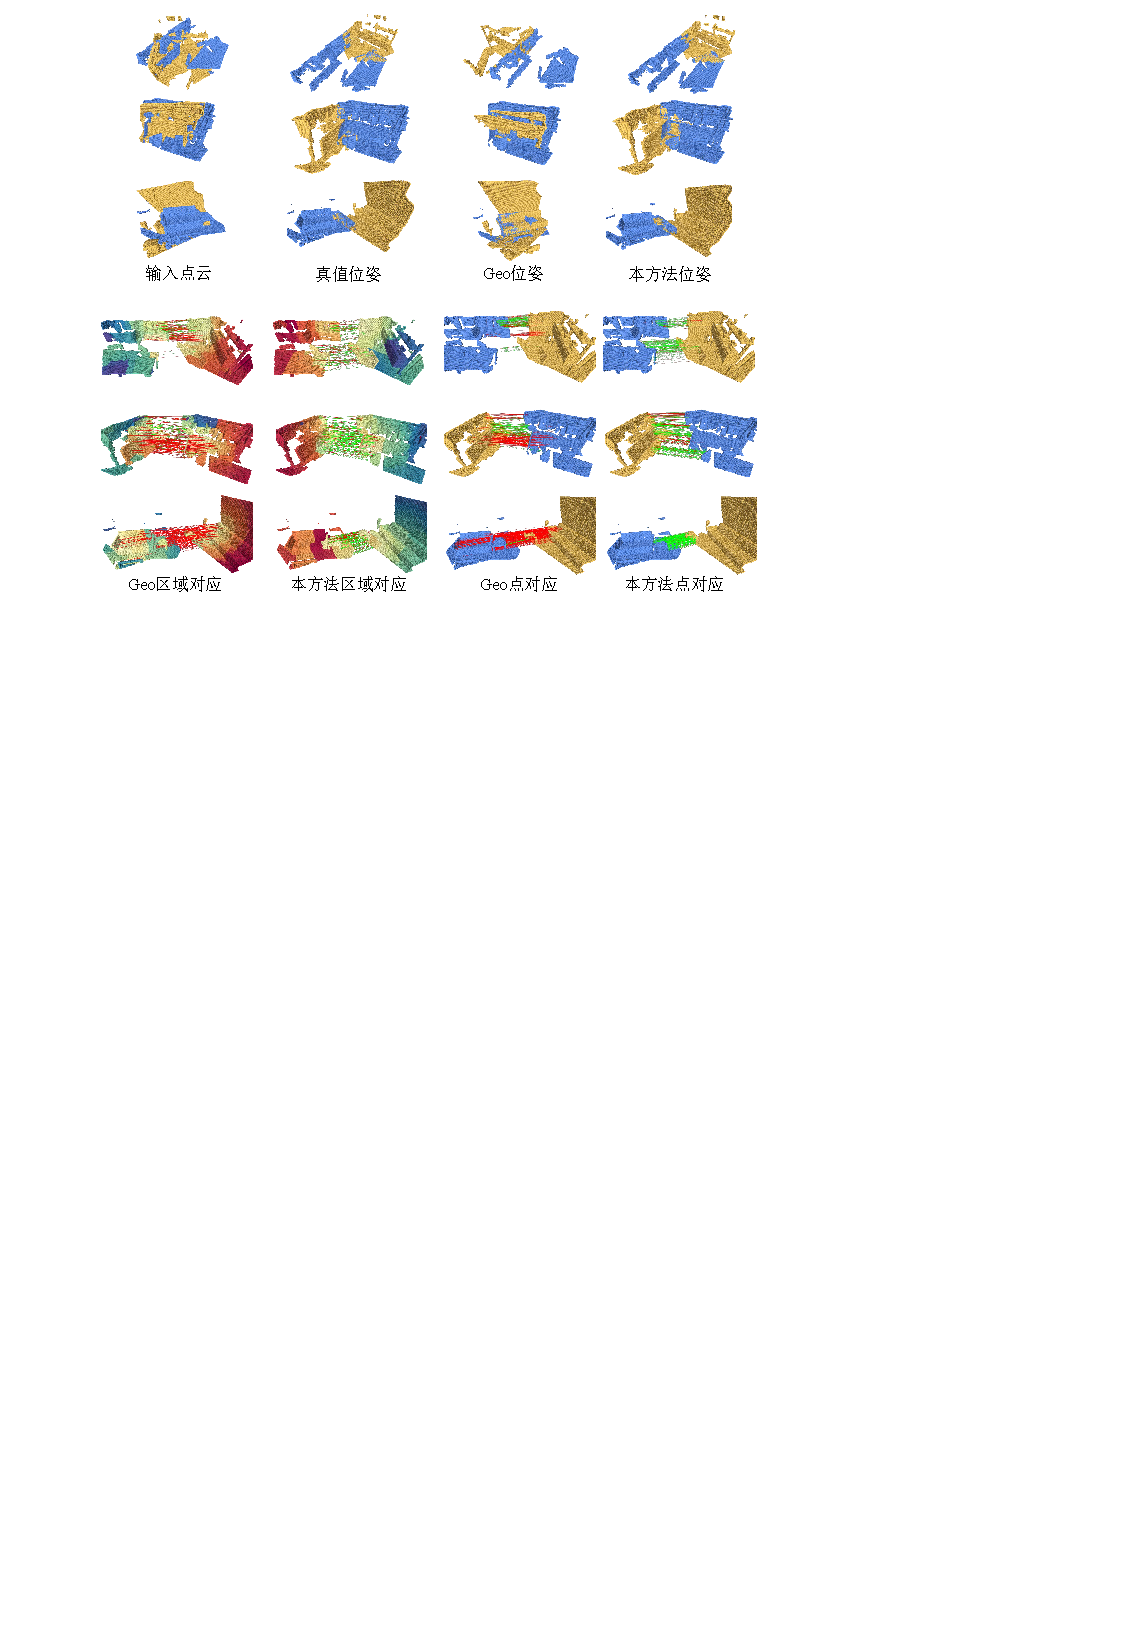
\includegraphics[width = \textwidth]{my/figure/3-5.pdf}
        \bicaption[\xiaosi 第三章方法和Geo在3DLoMatch上的可视化比较]{\wuhao 本方法和Geo在3DLoMatch上的可视化比较}{\wuhao Comparison of our method and Geo on the 3DLoMatch}
        \label{fig:cor_geo}
    \end{figure}
    \vspace{-0.35cm}

    (2)弱几何区域的比较。
    本文还在图\ref{fig:low_geometry}中显示了弱几何重叠区域的可视化结果。
    弱几何重叠区域在真实场景中非常常见,例如前两行的垂直平面和第三行的水平面。在这些弱几何区域中找到正确的对应关系并非易事。如图\ref{fig:low_geometry}所示,最先进的Geo方法在这三个例子上都会存在的前后颠倒问题。这是因为弱几何区域内的几何结构非常弱,以至于只能提取较少的具有差异性的特征来获得对应。通过本研究提出的关于锚点的选择性几何嵌入,本方法可以获得优越的性能。

    \vspace{-0.1cm}
    \begin{figure}[h]
        \centering
        \includegraphics[width = \textwidth]{my/figure/3-6.pdf}
        \bicaption[\xiaosi 弱几何区域情况下与Geo的比较]{\wuhao 弱几何区域情况下与Geo的比较}{\wuhao The comparison of registration on low-geometry region against Geo}
        \label{fig:low_geometry}
    \end{figure}
    \vspace{-0.35cm}
    % 3DMatch和3DLoMatch的更多配准结果如图\ref{qualitative_registration_results}所示。输入源点云和目标点云、真值配准、Geo的配准以及我们的结果显示在(a)到(d)列中。
    % 前三行是3DMatch的配准,其余行是3DLoMatch的结果。我们可以看到,我们的方法对于这些具有挑战性的情况是稳健的,在不同的重叠比下存在大量外观相似的区域。这些定性结果进一步验证了我们方法的有效性。
    % \begin{figure}[h]
    %     \centering
    %     \includegraphics[width = \textwidth]{my/figure/3-7.pdf}
    %     \caption{\wuhao The 3DMatch和3DLoMatch上的配准结果可视化。}
    %     \wuhao Fig.3-7 visualization of registration results on 3DMatch and 3DLoMatch.
    %     \label{qualitative_registration_results}
    % \end{figure}

    \subsection{KITTI实验}
    \subsubsection{数据集与评价指标}
    KITTI是一个由11个室外场景序列组成的点云数据集。本文取序列0-5作为训练集,6-7作为验证集,8-10作为测试集。同时使用ICP算法在给定的GPS定位上进一步微调真值变换矩阵,在评估阶段使用间距至少为10m的点云对。\par
    本实验主要采用相对旋转误差(RRE)、相对平移误差(RTE)和配准召回率(RR)三个评估指标来评估模型的性能。
    % 相对旋转误差是预测配准结果与真实配准值之间的测地线距离。相对平移误差是预测配准结果和真实配准值之间的欧氏距离。
    与3DMatch和3DLoMatch的配准召回率不同,此处的配准召回率表示相对旋转误差和相对平移误差小于各自阈值的点云对的比例。\par
    \subsubsection{与最先进技术的比较}
    在KITTI数据集上,本文将基于LGR的方法与目前最先进的3DFeat-Net、FCGF、D3Feat、SpinNet、Predator、CoFiNet和Geo方法进行了比较。如表\ref{tab:kitti},虽然本方法在相对旋转误差方面表现一般,但本文基于LGR的模型在相对平移误差上实现了SOTA性能,比基于LGR的Geo和基于RANSAC的Predator低了0.6cm。实验表明,该模型在室外数据集上也具有一定的泛化能力。
    \begin{table}[h]
	\renewcommand{\arraystretch}{1}
    \centering
    \setlength{\tabcolsep}{7mm}{
    \bicaption[\xiaosi 最先进的方法和本方法在KITTI数据集上的性能比较。]{\wuhao 最先进的方法和本方法在KITTI数据集上的性能比较}{\wuhao Comparisons between the SOTA and this method on the KITTI}
    \label{tab:kitti}
    \wuhao

    \begin{tabular}{lccc}
    \toprule[1.5pt]
    Model          &RTE(cm)        &RRE($^\circ$) &RR(\%)
    \\ \hline
    3DFeat-Net
    & 25.9         & \ul{0.25}     & 96.0 
    \\
    FCGF
    & 9.5          & 0.30          & 96.6
    \\
    D3Feat
    & 7.2          & 0.30          & \textbf{99.8}
    \\
    SpinNet
    & 9.9          & 0.47          & \ul{99.1}
    \\
    Predator
    & \ul{6.8}     & 0.27          & \textbf{99.8}
    \\
    CoFiNet
    & 8.2          & 0.41          & \textbf{99.8}
    \\
    Geo(Ransac-50k)
    & 7.4          & 0.27          & \textbf{99.8}
    \\
    Geo(LGR)
    & \ul{6.8}     & \textbf{0.24} & \textbf{99.8}
    \\
    %Ours (Ransac-50k) & 9.6          & 0.33          & \textbf{99.8} \\
    Ours(LGR)
    & \textbf{6.2} & 0.30          & \textbf{99.8}
    \\
    \bottomrule[1.5pt]
    \end{tabular}
    }
\end{table}

    % 更多的可视化结果显示在图\ref{MGReg_ki}中。很明显,我们提出的方法允许对室外点云进行准确的配准。
    % \begin{figure}[h]
    %     \centering
    %     \includegraphics[width = \textwidth]{my/figure/3-8.pdf}
    %     \caption{\wuhao KITTI数据集配准结果的可视化.}
    %     \wuhao The visualization of registration  on KITTI odometry.
    %     \label{MGReg_ki}
    % \end{figure}

    \subsection{消融实验}
    本节设计了消融实验来分析网络中一些超参数和模块的有效性。消融实验使用的数据集为3DMatch和3DLoMatch,且使用局部到全局的配准(LGR)方法来计算变换矩阵。为了评估超点对应的质量,本节引入一个超点匹配的评价指标超点内点率(PIR),用来表示预测的超点对应之间的实际重叠率。\par

    \subsubsection{锚点定位模块的效果}
    如表\ref{tab:ablation_anchor_way},锚点定位模块可以有效增强几何嵌入的作用,进一步提高点云配准结果。在3DMatch数据集上,与Top-K选择显著锚点的方法相比,NMS的锚点定位模块可将超点内点率、特征匹配召回率、内点率和配准召回率分别提高0.7\%、0.6\%、0.1\%和0.2\%。在3DLoMatch上的提升更加明显,其中配准召回率能够提升1.8\%。
    \begin{table}[htp]
	\renewcommand{\arraystretch}{1}
    \centering
    \bicaption[\xiaosi 锚点定位模块消融实验]{\wuhao 锚点定位模块消融实验}{\wuhao Ablation experiments of the anchor location}\label{tab:ablation_anchor_way}
    \wuhao
    \begin{tabular}{ccccccccc}
    \toprule[1.5pt]
    \multirow{2}{*}{Model} & \multicolumn{4}{c}{3DMatch}  & \multicolumn{4}{c}{3DLoMatch} \\
    &{PIR} &{FMR} &{IR} &{RR}
    &{PIR} &{FMR} &{IR} &{RR}    \\ \hline
    {Top-K} & 85.8 & 97.7 & 70.8 & 91.5 & 54.3 & 86.3 & 43.5 & 73.3 \\
    {NMS}     & 86.5 & 98.3 & 70.9 & 91.7 & 55.7 & 86.5 & 44.1 & 75.1 \\ \bottomrule[1.5pt]
    \end{tabular}
\end{table}
    在使用Top-K方法选择锚点对应关系时,可能会有多个锚点相互靠近,导致这些锚点无法一定的几何结构,更严重的是可能多个锚点在空间中的聚集性会使得多个锚点的退化为一个锚点,从而削弱了选择性几何嵌入模块的几何嵌入效果。
    本节还在图\ref{fig:anchor_way}中比较了使用不同锚点选择方式的配准结果和对应关系可视化。可以观察到使用锚点定位模块能够产生更加稀疏的区域对应和点对应,同时这些对应关系的正确性也能够有所保证,这有助于更准确的配准结果。\par

    \vspace{-0.1cm}
    \begin{figure}[H]
        \centering
        \includegraphics[width = \textwidth]{my/figure/3-7.pdf}
        \bicaption[\xiaosi NMS与Top-K锚点选择方法的配准结果的比较]{\wuhao NMS与Top-K锚点选择方法的配准结果的比较}{\wuhao Comparison of registration results using NMS and Top-K}
        \label{fig:anchor_way}
    \end{figure}
    \vspace{-0.35cm}

    \subsubsection{选择几何嵌入模块的效果}
    为了研究所提出的选择性几何嵌入模块的有效性,本节将其与仅使用自注意机制编码超点距离特征的基本模型进行比较。表\ref{tab:ablation_embedding}中的ED和EA分别表示距离嵌入和角度嵌入。通过在交叉注意上增加距离嵌入(+ED),3DMatch和3DLoMatch上的配准召回率分别提高了1\%和2.1\%。在此基础上进一步整合角度信息(+EA \& ED),3DMatch和3DLoMacth上的内点率分别提高了0.8\%和1.7\%。PIR也分别提高了1.9\%和1.5\%。更重要的是在3DLoMatch上的配准召回率也有0.9\%的提高。这意味着添加角度信息允许更准确的区域和点对应。因此,配准召回实现了最佳性能。该实验验证了选择性几何嵌入模块能够在真实的室内场景中提供有效的区分信息,基于锚点对应的点云间信息交互是有效的。\par
    \begin{table}[htp]
	\renewcommand{\arraystretch}{1}
    \centering
    \bicaption[\xiaosi 距离和角度嵌入对模型的影响]{\wuhao 距离和角度嵌入对模型的影响}{\wuhao The effect of distance and angle embedding on the model}\label{tab:ablation_embedding}
    \wuhao
    \begin{tabular}{lcccccccc}
    \toprule[1.5pt]
    \multicolumn{1}{c}{\multirow{2}{*}{Model}}
    & \multicolumn{4}{c}{3DMatch}
    & \multicolumn{4}{c}{3DLoMatch} \\
    \multicolumn{1}{c}{}
    & PIR   & FMR   & IR    & RR   & PIR   & FMR   & IR    & RR    \\ \hline
    baseline
    & 84.9  & 98.0  & 69.1  & 90.7 & 50.6  & 85.8  & 40.3  & 72.1  \\ 
    +ED
    & 84.6  & 98.3  & 70.1  & 91.7 & 54.2  & 86.8  & 42.4  & 74.2  \\ 
    +EA \& ED
    & 86.5  & 98.3  & 70.9  & 91.7 & 55.7  & 86.5  & 44.1  & 75.1  \\
    \bottomrule[1.5pt]
    \end{tabular}
\end{table}

    \subsubsection{基于迭代优化的显著锚更新效果}
    如表\ref{tab:ablation_iteration},在3DLoMatch上,迭代次数为2时的配准召回率比迭代次数为1的配准召回率高1.5\%,迭代次数为3的性能比迭代次数为2的性能低1\%。本文分析,随着迭代次数的增加,锚点的采样在一些不同的区域。

    当重叠率较低时,锚点不可避免地会集中。锚点集中后,嵌入的特征失去了差异,导致性能下降。这一点可以从\ref{tab:ablation_iteration}中的3DMatch实验中得到验证。当重叠率较高时,锚点分布相对均匀,不会造成性能下降。

    \begin{table}[h]
	\renewcommand{\arraystretch}{1}
    \centering
    \bicaption[\xiaosi 迭代次数对模型的影响]{\wuhao 迭代次数对模型的影响}{\wuhao The effect of the number of iterations on the model}\label{tab:ablation_iteration}
    \wuhao
    \begin{tabular}{ccccccccc}
    \toprule[1.5pt]
    \multicolumn{1}{l}{\multirow{2}{*}{Iteration}} 
    & \multicolumn{4}{c}{3DMatch}
    & \multicolumn{4}{c}{3DLoMatch} \\
    \multicolumn{1}{l}{}
    &{PIR} &{FMR} &{IR} &{RR}   
    &{PIR} &{FMR} &{IR} &{RR}    \\ \hline
    1
    & 75.1  & 98.8  & 64.4  & 91.3 & 44.6  & 87.8  & 37.1  & 73.6  \\
    2
    & 86.5  & 98.3  & 70.9  & 91.7 & 55.7  & 86.5  & 44.1  & 75.1  \\
    3
    & 87.2  & 97.9  & 71.8  & 91.4 & 57.3  & 86.6  & 45.3  & 74.1  \\
    \bottomrule[1.5pt]
    \end{tabular}
\end{table}

    本文还在图\ref{fig:ablation_iteration}中可视化源点云和目标点云中锚点的位置。蓝色球体是执行IOSAU之前的锚点位置,橙色球体是执行IOSAU之后的锚点位置。可以看到最初的锚点位于那些弱几何区域,如图\ref{fig:ablation_iteration}中第一行的两个例子中的桌面。但是,在进行基于迭代的优化更新后,可以看到更新后的锚点位于显著区域,如角落或尖锐的边界。这样,超点相对于显著锚点的几何嵌入具有明显的区别性,可以提高特征的区别度。

    \vspace{-0.1cm}
    \begin{figure}[h]
        \centering
        \includegraphics[width = \textwidth]{my/figure/3-8.pdf}

        \captionsetup{margin = {1.6cm, 1.6cm}}
        \bicaption[\xiaosi 基于迭代优化显著锚点更新前后源点云和目标点云中锚点位置的可视化]{\wuhao 基于迭代优化显著锚点更新前后源点云和目标点云中锚点位置的可视化
        % 。(a)1号源点云;(b) 1号目标点云;(c) 2号源点云;(d) 2号目标点云;(e) 3号源点云;(f) 3号目标点云;(g) 4号源点云;(h) 4号目标点云
        }{\wuhao Visualization of the location of anchor points in the source and target point clouds before and after iteration-based optimisation salient anchor updating
        % .(a) No. 1 source point cloud; (b) No. 1 target point cloud; (c) No. 2 source point cloud; (d) No. 2 target point cloud; (e) No. 3 source point cloud; (f) No. 3 target point cloud; (g) No. 4 source point cloud; (h) No. 4 target point cloud
        }
        \label{fig:ablation_iteration}
        % The blue spheres are the initial anchors before IOSAU. The red ones are the salient anchors after IOSAU.
    \end{figure}
    \vspace{-0.35cm}

    \section{本章小结}
    本文提出了一种基于显著锚点几何信息嵌入的鲁棒点云配准方法。利用分布稀疏且保持一定几何结构的锚点,选择性嵌入锚点与超点间的距离和角度的几何特征,增强特征间的差异性,实现精确的超点匹配。为了将最明显的信息融合到特征中,本章还提出了一种基于迭代优化的显著锚点更新,以实现最有效和最准确的几何嵌入。
    该方法以锚点对应为媒介,在源点云和目标点云之间交换几何信息。即使是在非重叠部分的外观相似区域,以及重叠部分的几何形状较弱的区域也能通过嵌入显著锚点对应相关的上下文信息实现准确可靠的区域对应。在室内和室外基准上进行的大量定量和定性实验验证了本章方法的有效性。